\documentclass[
	classe=$2^{de}$,
	headerTitle=Évaluation\space Chapitre\space 1,
	surFeuille
]{évaluation}

\usepackage{tcolorbox}
\usetikzlibrary{calc}

\title{Évaluation : Règles et outils de calcul (sujet A)}
\date{30 septembre 2022}

\begin{document}

\maketitle

\begin{tcolorbox}
	Cette évaluation est à rendre sur une feuille simple ou double.

	Ne pas oublier de mettre son nom et prénom sur sa copie, ainsi que le sujet (A ou B).

	La calculatrice est \textbf{interdite} ! \\

	Tous les résultats sont à donner sous forme \uline{d'entier} ou de \uline{fraction simplifiée}.
\end{tcolorbox}

\begin{exercice}
	Donner toutes les solutions des équations suivantes :
	\begin{multicols}{2}
		\begin{enumerate}
			\item $9x + 7 = 16$
			\item $3x + 2 = 9x - 6$
			\item $|x - 2| = 5$
			\item $|x + 3| = 6 × 7 - 40$
		\end{enumerate}
	\end{multicols}
\end{exercice}

\begin{exercice}
	Pour chaque phrase ci-dessous, répondre par vrai ou faux, en justifiant :
	\begin{enumerate}
		\item $6$ est une solution de l'équation $5x + 2 = 32$.
		\item $-2$ est une solution de l'équation $7x - 9 = -14$.
		\item $-1$ est une solution de l'inéquation $-2x > 6x + 5$.
		\item $6$ est une solution de l'équation $|3x - 20| + 7 × 3 = 23$.
		\item $-10$ est une solution de l'équation $|2x + 3 × 6| = 19 - 10 × 2$.
	\end{enumerate}
\end{exercice}

\begin{exercice}
	\begin{center}
		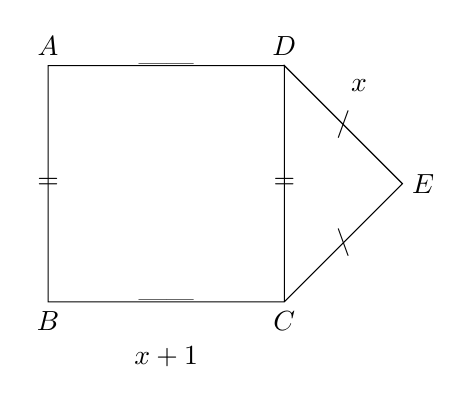
\begin{tikzpicture}
			\coordinate (A) at (0,0);
			\coordinate (B) at (0,-3);
			\coordinate (C) at (3,-3);
			\coordinate (D) at (3,0);
			\coordinate (E) at (4.5,-1.5);

			\foreach \p/\dir in {A/above,B/below,C/below,D/above,E/right} {
					\node[\dir] at (\p) {$\p$};
				}

			\draw (C)
			-- node[midway] {=} (D)
			-- node[midway] {/} node[midway,yshift=0.5cm,xshift=0.2cm] {$x$} (E)
			-- node[midway] {\textbackslash} (C)
			-- node[midway] {||} node[midway,yshift=-0.7cm] {$x + 1$} (B)
			-- node[midway] {=} (A)
			-- node[midway] {||} (D);
		\end{tikzpicture}
	\end{center}

	\begin{enumerate}
		\item Si le périmètre du carré $ABCD$ est égal au périmètre du triangle $CDE$, quelle équation vérifie $x$ ? % 4x + 4 = 3x + 1
		\item Donner la solution de cette équation. % x = -3
		      Peut-on construire cette figure ? % Et non.
	\end{enumerate}
\end{exercice}

\begin{exercice}
	On considère les expressions $A = \dfrac{3x}{5 × (x - 3)}$ et $B = \dfrac{-4x + 8}{-3 × 5 - 10}$.
	\begin{enumerate}
		\item Calculer la valeur de $A$ et de $B$ pour $x = 2$, puis pour $x = 8$. % 
		\item En utilisant la première question, donner une solution de l'équation $\dfrac{3x}{5 × (x - 3)} = \dfrac{-4x + 8}{-3 × 5 - 10}$.
	\end{enumerate}
\end{exercice}

\begin{exercice}
	Soit $X$ un point sur une droite graduée.

	En partant de $X$, on suit les instructions suivantes :
	\begin{itemize}
		\item Se déplacer de $6$ unités vers la gauche.
		\item Diviser sa distance à l'origine par $3$.
		\item Se déplacer de $5$ unités vers la gauche.
	\end{itemize}

	Après avoir suivi ces instructions, on se retrouve au point d'abscisse $7$.

	Quelle était la position du point $X$ ?
\end{exercice}

\end{document}